\section{Stabilizer}
In order to prove the applicability of the discussed stabilizer architecture, different experiments were carried out. The aim of this experiments is to show the feasibility of the model-based controller designed in \ref{chap:control_sec:stabilizer}. Only the ankle strategy is considered in this work applied in the sagittal plane when the robot is in double support phase. Humanoid robot TEO from Universidad Carlos III of Madrid is the subject of all experiments.

\subsection{Position control}
In order to prove the model-based position controller, the model parameters obtained in \eqref{eq:LQRparameters} \eqref{eq:LQRgain} are used. The stabilizer is designed to control the ZMP position through commanding different angular positions to robot joint ankles. 

\textcolor{red}{Incluir diagrama control posicion}

In Figure [], it is shown the control diagram. Here, the predictive model estimates a position of the ZMP point, called as $ZMP_{model}$, from the F-T sensor information ($ZMP_{FT}$) and the desired or reference $ZMP_{ref}$. The estimated ZMP is the control signal sent to the robot ankle joints, but position has to be converted to angular units.

In order to obtain the angular-position units relation we did several experimental trials. Giving to ankle joints angles from 0 to 5 degrees, in 0.5 increment, the measured global ZMP (according to ZMP double-support equation \eqref{eq:xZmpDoubleSupport} and removing sensors offset) has a linear relation with the set angle. Figure \ref{fig:angle_zmp_relation} shows the obtained average relation expressed as:

\begin{equation}
ZMP_{F-T} = q \cdot \theta_A
\end{equation}

where $ZMP_{F-T}$ is the measured ZMP, $\theta_A$ is the angle of the ankle joints and $q=-0.0135 \frac{m}{deg}$.

\begin{figure}[!hbt]
\centering
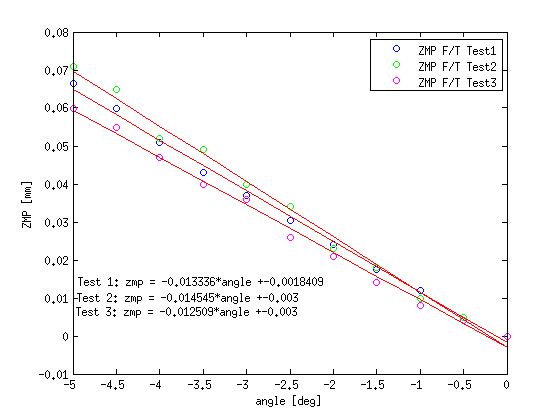
\includegraphics[scale=0.5]{angle_zmp_relation3.png}
\caption{Experimental $\theta_A - ZMP_{F-T}$ relation}
\label{fig:angle_zmp_relation}
\end{figure}

The obtained converter factor ought to be useful reverse in order to obtain the required angle to reach a desired ZMP. But experimentally, taking the relation above, the $ZMP_{F-T}$ is different from the setpoint value. Several test were done from 0 to 0.1 m in 0.005 m increments. Results obtained are shown in Figure \ref{fig:ZMPerror}. One can see that 



\begin{figure}[!hbt]
\centering
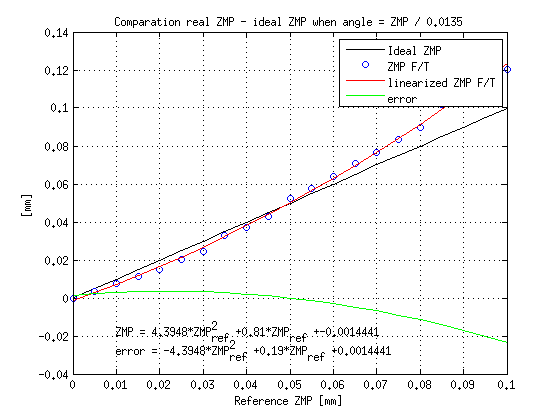
\includegraphics[scale=0.5]{zmp_real_ideal2.png}
\caption{Measured ZMP error}
\label{fig:ZMPerror}
\end{figure}

\subsection{Velocity control}

\subsection{Model changes}

\subsection{ZMP areas}
As mentioned before, the robot can recover its balance or not depending on the ZMP position and which parts of its body are compensating the fall down. The ankle strategy should be enough to recover balance from a low disturbance. In order to decide this strategy limit, some experimental trials have been done. 

Firstly, the ankle strategy ZMP limit was obtained starting from an upright position -blocking arms, neck and trunk joints-, and giving increasing ZMP reference positions. After \textcolor{red}{five} tests, the average ZMP limit forwards is \textcolor{red}{¿? m} and backwards \textcolor{red}{¿? m}. The great difference of ZMP limit between forwards and backwards is mainly due to the shape of the supporting area (the sole). The mechanical design of the robot feet and legs, make that forwards there is a greater surface in contact with the ground because the center of the ankle joint is displaced rearwards of the center of the sole (see Appendix \ref{app:footDraw}).

\textcolor{red}{Quizá una gráfica de los experimentos y el limite en cada uno de ellos con la media?}

Other experiment carried out is related to the maximum torque of the ankle motors. Brushless motors installed at ankle joints are ......... The highest torque the motors can exert is the maximum angle, thus the maximum ZMP position that ankle joints themselves can reach.


\textcolor{red}{Al final, una figura con la huella del pie y las zonas delimitadas.}

